\section{pbdR}
\makesubcontentsslides

\subsection{The pbdR Project}
\makesubcontentsslidessec

\begin{frame}{\pbdR Interfaces to Libraries: Sustainable Path}
  \vspace{-1ex}
  \centering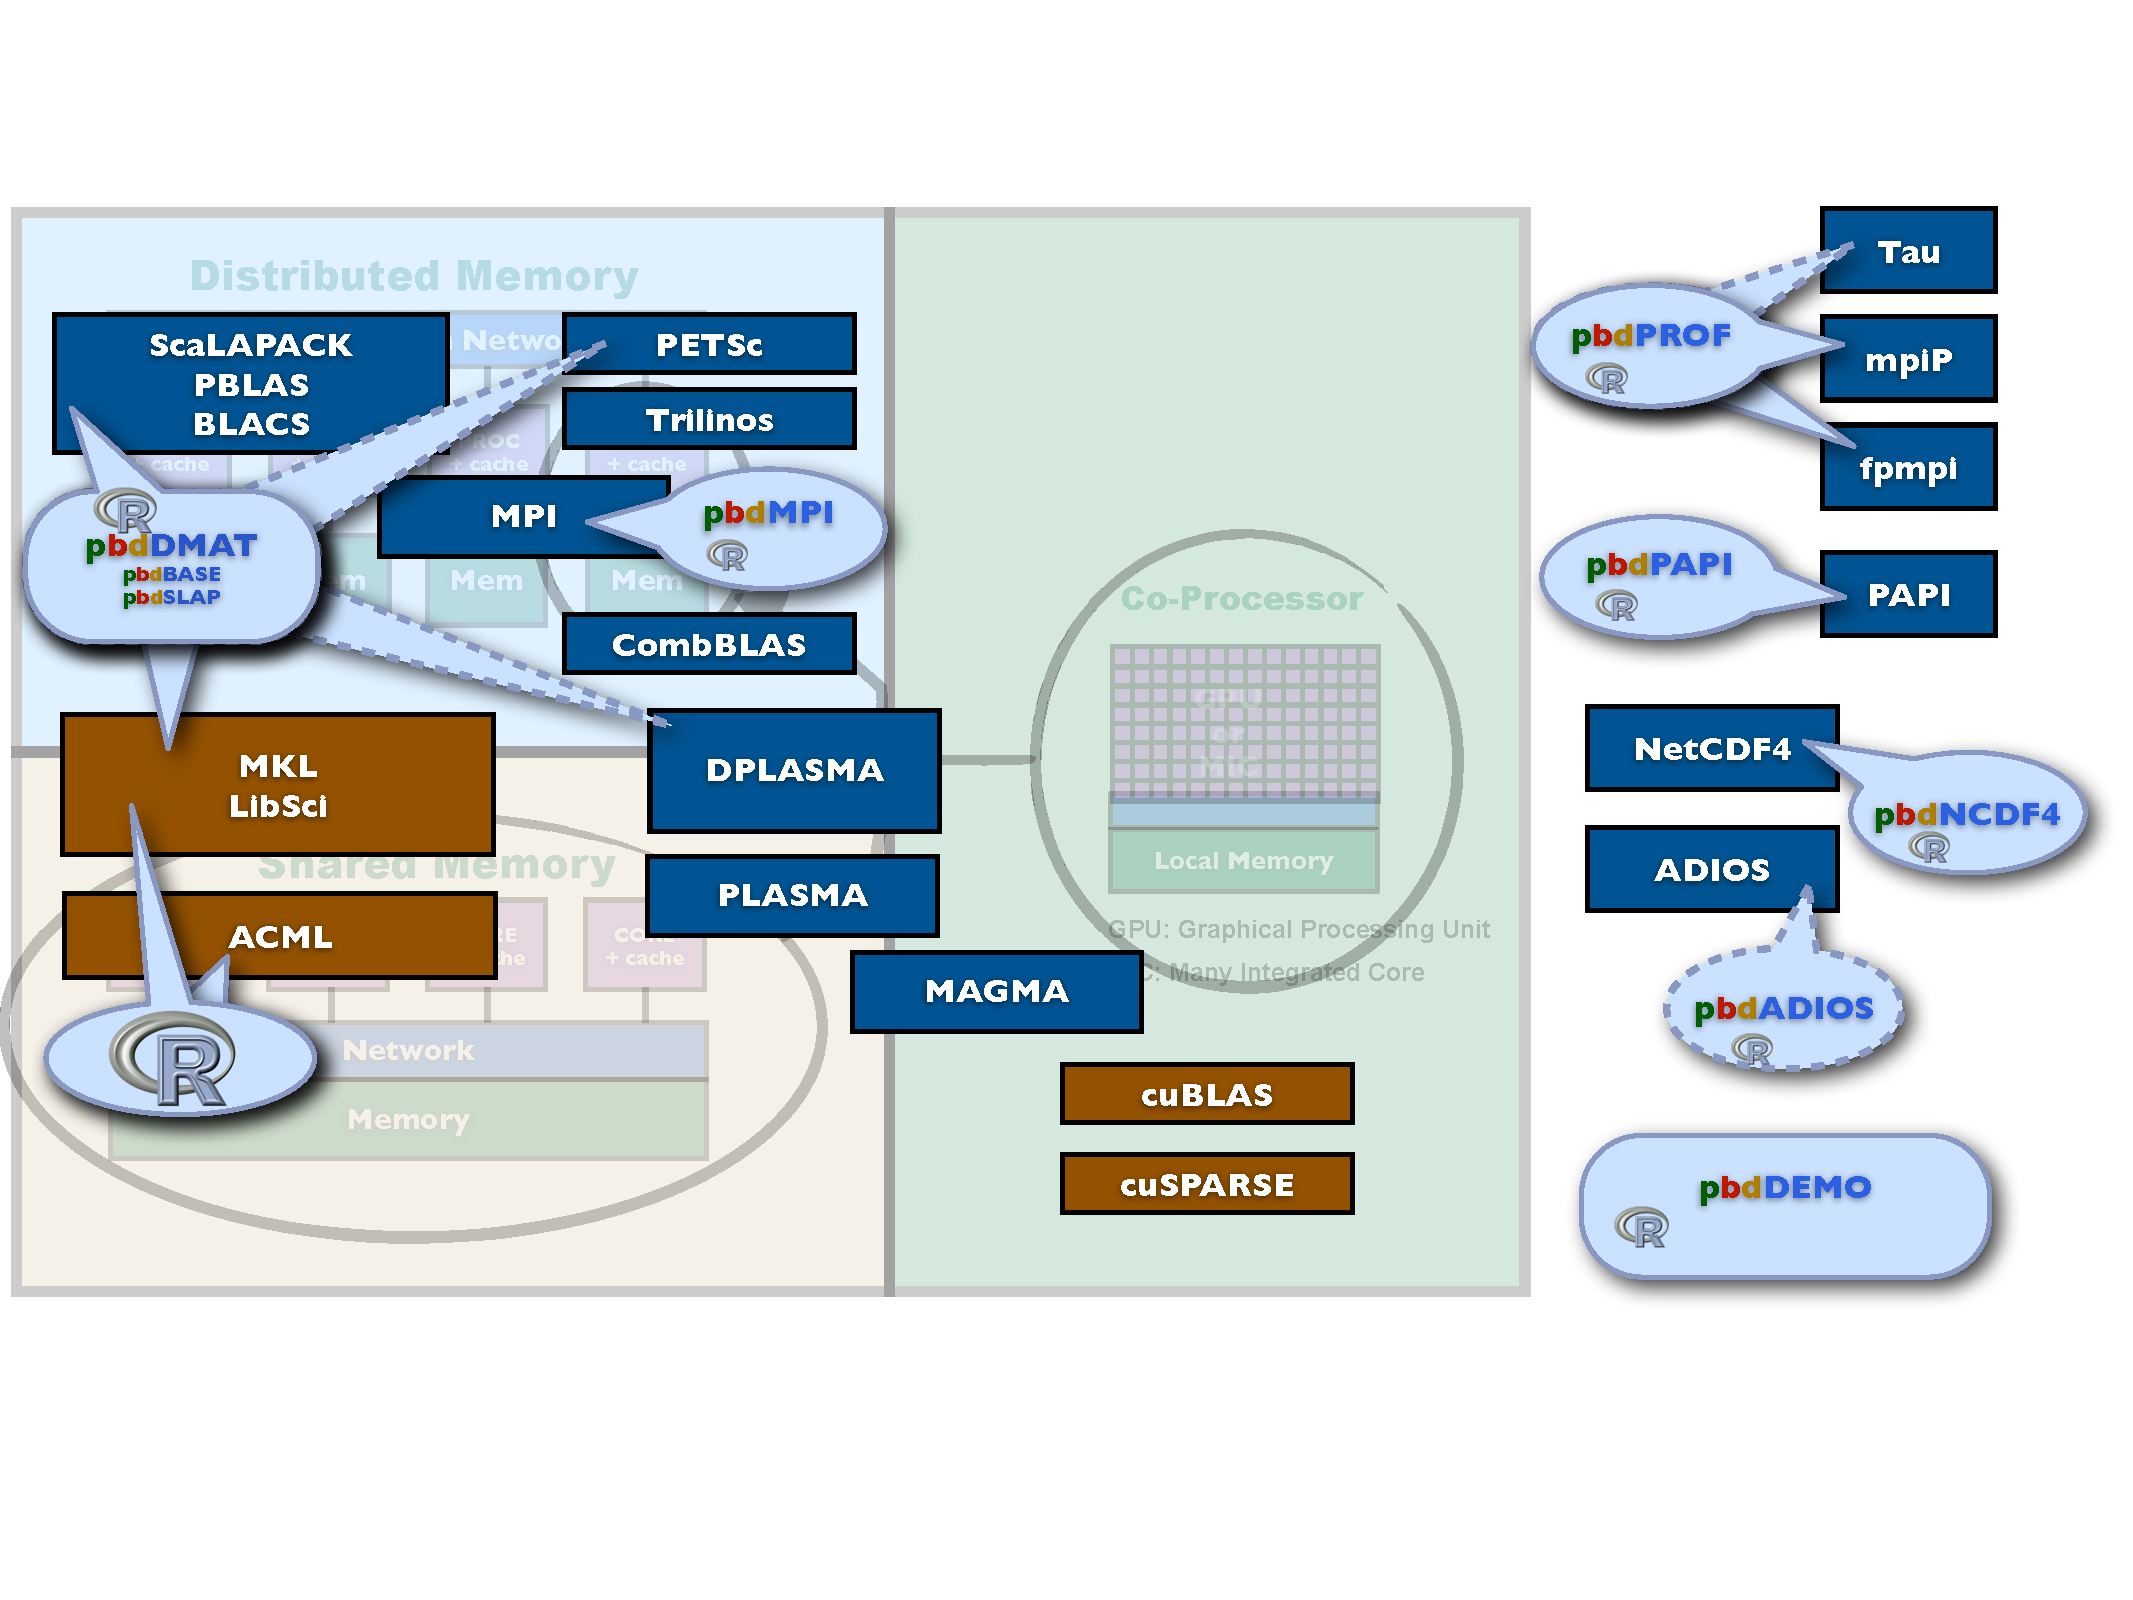
\includegraphics[trim=0cm 5cm 0cm 3cm,clip=true,width=0.85\textwidth]
  {../common/pics/hardware/ParallelHardware27.pdf}
  \scriptsize
  \begin{block}{Why use HPC libraries?}
    \begin{itemize}[<+-|alert@+>]
    \item The HPC community is 30 years beyond ``embarrassingly parallel.''
    \item \emph{They're tested.} \emph{They're
        fast.}  \emph{They're scalable.}
    \item Many science communities are invested in their API.
    \item You're not going to beat Jack Dongarra's lab at dense linear
      algebra!
    \end{itemize}
  \end{block}
\end{frame}

\subsection{pbdMPI}
\makesubcontentsslidessec

\begin{frame}
  \begin{block}{pbdMPI: Simplified, Extensible, and Fast Communication Operations}\pause
    \begin{itemize}
    \item S4 methods for collective communication: extensible to other
      \R objects.
    \item Default methods (like \code{Robj} in \pkg{Rmpi}) check for
      data type: safe for general users.
    \item API is simplified: defaults in control objects.
    \item Array and matrix methods without serialization: faster than
      \pkg{Rmpi}.
    \end{itemize}
    \begin{center}
      \vspace{0.2cm}\scriptsize
      \begin{tabular}{ll} \hline\hline
        \pkg{pbdMPI} (S4) & \pkg{Rmpi}                \\ \hline
        \code{allgather}    & \code{mpi.allgather},
        \code{mpi.allgatherv},
        \code{mpi.allgather.Robj} \\
        \code{allreduce}    & \code{mpi.allreduce}      \\
        \code{bcast}        & \code{mpi.bcast},
        \code{mpi.bcast.Robj}     \\
        \code{gather}       & \code{mpi.gather},
        \code{mpi.gatherv},
        \code{mpi.gather.Robj}    \\
        \code{recv}         & \code{mpi.recv},
        \code{mpi.recv.Robj}      \\
        \code{reduce}       & \code{mpi.reduce}         \\
        \code{scatter}      & \code{mpi.scatter},
        \code{mpi.scatterv},
        \code{mpi.scatter.Robj}   \\
        \code{send}         & \code{mpi.send},
        \code{mpi.send.Robj}      \\ \hline \hline
      \end{tabular}
    \end{center}
  \end{block}
\end{frame}

\begin{frame}[fragile]
  \begin{block}{pbdMPI: Does the Right Thing for You}\pause
    \begin{minipage}[t]{.475\textwidth}
      \begin{lstlisting}[title=Rmpi]
# int
mpi.allreduce(x, type=1)
# double
mpi.allreduce(x, type=2)
      \end{lstlisting}
    \end{minipage}
    \hfill
    \begin{minipage}[t]{.475\textwidth}
      \begin{lstlisting}[title=pbdMPI]
allreduce(x)
      \end{lstlisting}
      % \vspace{1em}
      % \hspace{1em}{\small S4. Batch only! (No spawning)}
    \end{minipage}
  \end{block}
  \begin{block}{Types in R}
    \vspace{-.2cm}
    \begin{lstlisting}
> is.integer(1)
[1] FALSE
> is.integer(2)
[1] FALSE
> is.integer(1:2)
[1] TRUE
    \end{lstlisting}
  \end{block}
\end{frame}

% \begin{frame}[fragile]{Single Program (SPMD): Runs Asynchronous Parallel}
%   \begin{exampleblock}{Rank Query Example}
%     \centering
%     \begin{lstlisting}[title=1\_rank.r]
% library(pbdMPI, quiet = TRUE)
% init()

% my.rank <- comm.rank()
% comm.print(my.rank, all.rank=TRUE)

% finalize()
%     \end{lstlisting}
%     \begin{columns}[t,onlytextwidth]
%       \begin{column}{0.62\textwidth}
%         \begin{lstlisting}[backgroundcolor=\color{white},keywordstyle=\color{black},
% title=Execute this batch script via:]
% mpirun -np 2 Rscript 1_rank.r
%         \end{lstlisting}
%       \end{column}
%       \hfill
%       \begin{column}{0.35\textwidth}
%         \begin{lstlisting}[title=Sample Output:]
% COMM.RANK = 0
% [1] 0
% COMM.RANK = 1
% [1] 1
%         \end{lstlisting}
%       \end{column}
%     \end{columns}
%   \end{exampleblock}
% \end{frame}

\subsection{pbdDMAT}
\makesubcontentsslidessec

\begin{frame}{Mapping a Matrix to Processors}
  \begin{block}{Processor Grid Shapes}
    \begin{table}[ht]
      \centering
      % \begin{subfigure}[b]{0.23\textwidth}
      %   \centering
      %   $\left[\begin{tabular}{l}
      %       0 \\ 1 \\ 2 \\ 3 \\ 4 \\ 5
      %     \end{tabular}\right]^T$
      %   \caption{$1\times 6$}
      % \end{subfigure}
      \begin{subfigure}[b]{0.23\textwidth}
        \centering
        $\left[\begin{tabular}{llllll}
            0 & 1 & 2 & 3 & 4 & 5
          \end{tabular}\right]$
        \vspace{1.5cm}
        \caption{$1\times 6$}
      \end{subfigure}%\hspace{-1cm}
      \begin{subfigure}[b]{0.23\textwidth}
        \centering
        $\left[\begin{tabular}{lll}
            0 & 1 & 2\\
            3 & 4 & 5
          \end{tabular}\right]$
        \caption{$2\times 3$}
      \end{subfigure}%
      \begin{subfigure}[b]{0.23\textwidth}
        \centering
        $\left[\begin{tabular}{ll}
            0 & 1 \\
            2 & 3\\
            4 & 5
          \end{tabular}\right]$
        \caption{$3\times 2$}
      \end{subfigure}
      \begin{subfigure}[b]{0.23\textwidth}
        \centering
        $\left[\begin{tabular}{l}
            0 \\ 1 \\ 2 \\ 3 \\ 4 \\ 5
          \end{tabular}\right]$
        \caption{$6\times 1$}
      \end{subfigure}
      \caption{Processor Grid Shapes with 6 Processors}\label{fig:gridshapes}
    \end{table}
  \end{block}
\end{frame}

\begin{frame}[shrink]
\begin{exampleblock}{2$\times$3 block-cyclic grid on 6 processors:
    Global view ``ddmatrix'' class}
\begin{align*}
x &= \left[
      \begin{array}{ll|ll|ll|ll|l}
      \color{g11}x_{11} & \color{g11}x_{12} & \color{g12}x_{13} & \color{g12}x_{14} & \color{g13}x_{15} & \color{g13}x_{16} & \color{g11}x_{17} & \color{g11}x_{18} & \color{g12}x_{19}\\
      \color{g11}x_{21} & \color{g11}x_{22} & \color{g12}x_{23} & \color{g12}x_{24} & \color{g13}x_{25} & \color{g13}x_{26} & \color{g11}x_{27} & \color{g11}x_{28} & \color{g12}x_{29}\\\hline
      \color{g21}x_{31} & \color{g21}x_{32} & \color{g22}x_{33} & \color{g22}x_{34} & \color{g23}x_{35} & \color{g23}x_{36} & \color{g21}x_{37} & \color{g21}x_{38} & \color{g22}x_{39}\\
      \color{g21}x_{41} & \color{g21}x_{42} & \color{g22}x_{43} & \color{g22}x_{44} & \color{g23}x_{45} & \color{g23}x_{46} & \color{g21}x_{47} & \color{g21}x_{48} & \color{g22}x_{49}\\\hline
      \color{g11}x_{51} & \color{g11}x_{52} & \color{g12}x_{53} & \color{g12}x_{54} & \color{g13}x_{55} & \color{g13}x_{56} & \color{g11}x_{57} & \color{g11}x_{58} & \color{g12}x_{59}\\
      \color{g11}x_{61} & \color{g11}x_{62} & \color{g12}x_{63} & \color{g12}x_{64} & \color{g13}x_{65} & \color{g13}x_{66} & \color{g11}x_{67} & \color{g11}x_{68} & \color{g12}x_{69}\\\hline
      \color{g21}x_{71} & \color{g21}x_{72} & \color{g22}x_{73} & \color{g22}x_{74} & \color{g23}x_{75} & \color{g23}x_{76} & \color{g21}x_{77} & \color{g21}x_{78} & \color{g22}x_{79}\\
      \color{g21}x_{81} & \color{g21}x_{82} & \color{g22}x_{83} & \color{g22}x_{84} & \color{g23}x_{85} & \color{g23}x_{86} & \color{g21}x_{87} & \color{g21}x_{88} & \color{g22}x_{89}\\\hline
      \color{g11}x_{91} & \color{g11}x_{92} & \color{g12}x_{93} & \color{g12}x_{94} & \color{g13}x_{95} & \color{g13}x_{96} & \color{g11}x_{97} & \color{g11}x_{98} & \color{g12}x_{99}\\
      \end{array}
\right]_{9\times 9}
\end{align*}
\begin{align*}
\text{Processor grid = }\left|
      \begin{array}{lll}
      \color{g11}0 & \color{g12}1 & \color{g13}2\\
      \color{g21}3 & \color{g22}4 & \color{g23}5
      \end{array}
\right| &=
\left|
      \begin{tabular}{lll}
      \color{g11}(0,0) & \color{g12}(0,1) & \color{g13}(0,2)\\
      \color{g21}(1,0) & \color{g22}(1,1) & \color{g23}(1,2)
      \end{tabular}
\right|
\end{align*}
\end{exampleblock}
\end{frame}


\begin{frame}[shrink]
\begin{exampleblock}{2$\times$3 block-cyclic grid on 6 processors:
    Local view ``ddmatrix'' class}
\begin{align*}
\left[
      \begin{array}{ll|ll}
      \color{g11}x_{11} & \color{g11}x_{12} & \color{g11}x_{17} & \color{g11}x_{18}\\
      \color{g11}x_{21} & \color{g11}x_{22} & \color{g11}x_{27} & \color{g11}x_{28}\\\hline
      \color{g11}x_{51} & \color{g11}x_{52} & \color{g11}x_{57} & \color{g11}x_{58}\\
      \color{g11}x_{61} & \color{g11}x_{62} & \color{g11}x_{67} & \color{g11}x_{68}\\\hline
      \color{g11}x_{91} & \color{g11}x_{92} & \color{g11}x_{97} & \color{g11}x_{98}\\
      \end{array}
\right]_{5\times 4}
\left[
      \begin{array}{ll|l}
      \color{g12}x_{13} & \color{g12}x_{14} & \color{g12}x_{19}\\
      \color{g12}x_{23} & \color{g12}x_{24} & \color{g12}x_{29}\\\hline
      \color{g12}x_{53} & \color{g12}x_{54} & \color{g12}x_{59}\\
      \color{g12}x_{63} & \color{g12}x_{64} & \color{g12}x_{69}\\\hline
      \color{g12}x_{93} & \color{g12}x_{94} & \color{g12}x_{99}\\
      \end{array}
\right]_{5\times 3}
\left[
      \begin{array}{ll}
      \color{g13}x_{15} & \color{g13}x_{16}\\
      \color{g13}x_{25} & \color{g13}x_{26}\\\hline
      \color{g13}x_{55} & \color{g13}x_{56}\\
      \color{g13}x_{65} & \color{g13}x_{66}\\\hline
      \color{g13}x_{95} & \color{g13}x_{96}\\
      \end{array}
\right]_{5\times 2}
\\
\left[
      \begin{array}{ll|ll}
      \color{g21}x_{31} & \color{g21}x_{32} & \color{g21}x_{37} & \color{g21}x_{38}\\
      \color{g21}x_{41} & \color{g21}x_{42} & \color{g21}x_{47} & \color{g21}x_{48}\\\hline
      \color{g21}x_{71} & \color{g21}x_{72} & \color{g21}x_{77} & \color{g21}x_{78}\\
      \color{g21}x_{81} & \color{g21}x_{82} & \color{g21}x_{87} & \color{g21}x_{88}\\
      \end{array}
\right]_{4\times 4}
\left[
      \begin{array}{ll|l}
      \color{g22}x_{33} & \color{g22}x_{34} & \color{g22}x_{39}\\
      \color{g22}x_{43} & \color{g22}x_{44} & \color{g22}x_{49}\\\hline
      \color{g22}x_{73} & \color{g22}x_{74} & \color{g22}x_{79}\\
      \color{g22}x_{83} & \color{g22}x_{84} & \color{g22}x_{89}\\
      \end{array}
\right]_{4\times 3}
\left[
      \begin{array}{ll}
      \color{g23}x_{35} & \color{g23}x_{36} \\
      \color{g23}x_{45} & \color{g23}x_{46} \\\hline
      \color{g23}x_{75} & \color{g23}x_{76} \\
      \color{g23}x_{85} & \color{g23}x_{86} \\
      \end{array}
\right]_{4\times 2}
\end{align*}
\begin{align*}
\text{Processor grid = }\left|
      \begin{array}{lll}
      \color{g11}0 & \color{g12}1 & \color{g13}2\\
      \color{g21}3 & \color{g22}4 & \color{g23}5
      \end{array}
\right| &=
\left|
      \begin{tabular}{lll}
      \color{g11}(0,0) & \color{g12}(0,1) & \color{g13}(0,2)\\
      \color{g21}(1,0) & \color{g22}(1,1) & \color{g23}(1,2)
      \end{tabular}
\right|
\end{align*}
\end{exampleblock}
\end{frame}

\begin{frame}[fragile]
  \begin{block}{\pbdR\ Example Syntax}
\vspace{-2ex}
  \begin{lstlisting}
x <- x[-1, 2:5]
x <- log(abs(x) + 1)
x.pca <- prcomp(x)
xtx <- t(x) %*% x
ans <- svd(solve(xtx))
  \end{lstlisting}
\vspace{-1ex}
  \begin{center}
  \emph{The above (and over 100 other functions) runs on 1 core with R \\
    or 10,000 cores with \pbdR ddmatrix class}
  \end{center}
\vspace{-2ex}
\begin{lstlisting}
> showClass("ddmatrix")
Class "ddmatrix" [package "pbdDMAT"]
Slots:
Name:     Data     dim    ldim   bldim   ICTXT
Class:  matrix numeric numeric numeric numeric
\end{lstlisting}
\vspace{-2ex}
\begin{lstlisting}
> x <- as.rowblock(x)
> x <- as.colblock(x)
> x <- redistribute(x, bldim=c(8, 8), ICTXT = 0)
\end{lstlisting}
  \end{block}
\end{frame}

% \begin{frame}[fragile]
%   \begin{block}{Covariance \hspace{2.1cm}Serial\hspace{0.5cm}Parallel}
%     \begin{minipage}{5cm}
%       \vspace{-1ex}
%       \begin{lstlisting}[backgroundcolor=\color{white},title=low-level]
% N <- nrow(X)
% mu <- colSums(X) / N
% X <- sweep(X, 2, mu)
% cX <- crossprod(X)/(N-1)
%       \end{lstlisting}
%       \vspace{-1ex}
%       \begin{lstlisting}[backgroundcolor=\color{white},title=high-level]
% cX <- cov(X)
%       \end{lstlisting}
%     \end{minipage}
%     \begin{minipage}{6.9cm}
%       \vspace{-1ex}
%       \begin{lstlisting}[title=low-level (row-block)]
% N <- allreduce(nrow(X))
% mu <- allreduce(colSums(X))/N
% X <- sweep(X, 2, mu)
% cX <- allreduce(crossprod(X))/(N-1)
%       \end{lstlisting}
%       \vspace{-1ex}
%       \begin{lstlisting}[title={\tt ddmatrix}]
% cX <- cov(X)
%       \end{lstlisting}
%     \end{minipage}
%   \end{block}
%   \begin{block}{Regression models}
%     \begin{minipage}{5cm}
%       \vspace{-1ex}
%       \begin{lstlisting}[backgroundcolor=\color{white},title=low-level]
% tX <- t(X)
% A <- tx %*% X
% B <- tx %*% Y
% ols <- solve(A, B)
%       \end{lstlisting}
%       \vspace{-1ex}
%       \begin{lstlisting}[backgroundcolor=\color{white},title=high-level]
% Lm.X <- lm.fit(X, Y)
%       \end{lstlisting}
%     \end{minipage}
%     \begin{minipage}{6.9cm}
%       \vspace{-1ex}
%       \begin{lstlisting}[title=low-level (row-block)]
% tX <- t(X)
% A <- allreduce(tx %*% X)
% B <- allreduce(tx %*% Y)
% ols <- solve(A, B)
%       \end{lstlisting}
%       \vspace{-1ex}
%       \begin{lstlisting}[title={\tt ddmatrix}]
% Lm.X <- lm.fit(X, Y)
%       \end{lstlisting}
%     \end{minipage}
%   \end{block}
% \end{frame}

% \subsection{Advanced R Profiling}
% \makesubcontentsslidessec

% \begin{frame}[fragile]
%   \small
%   \begin{block}{Profiling MPI codes with \textbf{pbdPROF}}
%   \begin{minipage}[t]{.58\textwidth}
%   \vspace{.2cm}
%   1. Rebuild \pbdR\ packages
% \vspace*{-.5cm}
% \begin{lstlisting}[language=shl,title=\ ]
% R CMD INSTALL pbdMPI_0.2-1.tar.gz \ --configure-args= \ "--enable-pbdPROF"
% \end{lstlisting}
% 2. Run code
% \vspace*{-.5cm}
% \begin{lstlisting}[language=shl,title=\ ]
% mpirun -np 64 Rscript my_script.R
% \end{lstlisting}

% 3. Analyze results
% \vspace{-.5cm}
% \begin{lstlisting}[title=\ ]
% library(pbdPROF)
% prof <- read.prof( "profiler_output.mpiP")
% plot(prof, plot.type="messages2")
% \end{lstlisting}
%   \end{minipage}
%   \hfill
%   \begin{minipage}[t]{.4\textwidth}
%   \vspace{0pt}
%     \centering
%     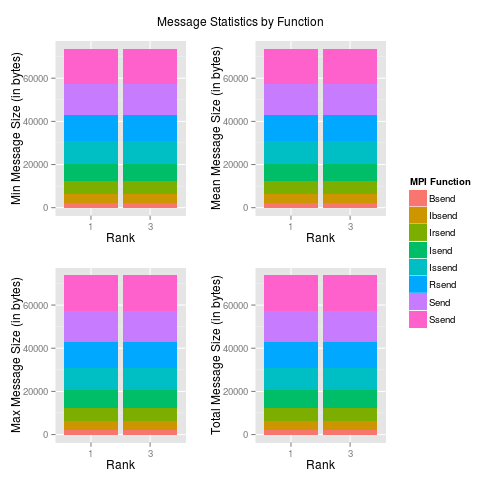
\includegraphics[scale=.25]{../common/pics/mpip}
%     \\[.1cm]
%     
\includegraphics[scale=0.3]{../common/pics/gsoc}
%   \end{minipage}
%   \centering
%   Supports fpmpi and mpiP.  Expanding to include support for TAU!
%   \end{block}
% \end{frame}

% \begin{frame}[fragile]
%   \small
%   \begin{block}{Profiling with \textbf{pbdPAPI}}
%     \begin{minipage}{.6\textwidth}
%       \begin{itemize}
%       \item Bindings for Performance Application Programming Interface (PAPI)
%       \item Gathers detailed hardware counter data.
%       \item High and low level interfaces
%       \end{itemize}
%     \end{minipage}
%     \begin{minipage}{.38\textwidth}
%       \centering
%       
\includegraphics[scale=0.12]{../common/pics/gsoc_2014}
%     \end{minipage}
%     \begin{center}
%       \begin{tabular}{ll} \hline\hline
%         Function & Description of Measurement \\ \hline
%         \code{system.flips()} & Time, floating point instructions, and Mflips \\
%         \code{system.flops()} & Time, floating point operations, and Mflops \\
%         \code{system.cache()} & Cache misses, hits, accesses, and reads \\
%         \code{system.epc()} & Events per cycle \\
%         \code{system.idle()} & Idle cycles \\
%         \code{system.cpuormem()} & CPU or RAM bound$^*$ \\
%         \code{system.utilization()} & CPU utilization$^*$ \\
%         \hline\hline
%       \end{tabular}
%     \end{center}
%   \end{block}
% \end{frame}

